\documentclass[runningheads]{llncs}
\usepackage[T1]{fontenc}
\usepackage[english]{babel}
\usepackage[backend=bibtex]{biblatex}
\addbibresource{main.bib}
\usepackage{graphicx}
\usepackage{amsmath,amssymb}
\usepackage{algpseudocode}
\usepackage{hyperref}
\usepackage{enumitem}
\usepackage{tikz}
\usepackage{caption}
\usepackage{booktabs} 
\usepackage{subcaption}
\usetikzlibrary{trees,positioning,arrows.meta,calc}
\usepackage{algorithm}




\begin{document}

\title{General Review of Hash-Based Signatures }

\author{Halil İbrahim Kaplan\inst{1}\orcidID{0009-0006-0120-6512}}
\authorrunning{Halil İbrahim Kaplan}

\institute{
Cryptanalysis Laboratory, TÜBİTAK BİLGEM, Kocaeli, Turkey\\
\email{halil.kaplan@tubitak.gov.tr}
}

\maketitle

\begin{abstract}
The advent of quantum computing threatens the security assumptions underpinning classical public-key cryptographic algorithms such as RSA and ECC. As a response, the cryptographic community has focused on developing quantum-resistant alternatives, with hash-based signature schemes emerging as a compelling option due to their reliance on well-understood hash functions rather than number-theoretic hardness assumptions. This paper presents a comprehensive review of hash-based signature schemes, including Lamport, WOTS, XMSS, $XMSS^{MT}$, and SPHINCS+, examining their structural design, key generation, signing, and verification processes. Emphasis is placed on their classification as stateful and stateless schemes, as well as their practical integration using Merkle trees and address structures. Furthermore, the paper analyzes several notable cryptanalytic attacks—such as intermediate value guessing, Antonov’s attack, multi-target attacks, and fault injection strategies—that pose risks to these constructions. By discussing both their strengths and vulnerabilities, this work highlights the viability of hash-based signatures as secure and efficient candidates for post-quantum digital signatures.

\keywords{Post-quantum cryptography \and Hash-based signatures \and XMSS \and SPHINCS+ \and Cryptanalysis}
\end{abstract}

\section{Introduction}

Hash-based signature (HBS) schemes have been known since the late 1970s, with early contributions by Lamport and Merkle. However, for many years, they remained theoretical constructs without widespread practical use, primarily due to their large signature sizes and, in the case of stateful schemes, complex key management requirements. This perception has shifted significantly with the emergence of post-quantum cryptography (PQC), which aims to develop cryptographic primitives that are resistant to quantum attacks.

The threat posed by quantum computers—particularly Shor's algorithm, which can break RSA and elliptic curve cryptography (ECC)—has led to renewed interest in HBS schemes. Unlike number-theoretic approaches, HBS algorithms rely solely on the security of cryptographic hash functions, which are believed to remain secure even in the presence of quantum adversaries.

This growing interest has been formalized through standardization efforts. The Internet Engineering Task Force (IETF) published RFC 8391 for the eXtended Merkle Signature Scheme (XMSS) in 2018, followed by the Leighton-Micali Signature (LMS) scheme. In parallel, the National Institute of Standards and Technology (NIST) provided parameter recommendations and, in 2022, selected the stateless scheme SPHINCS+ as a finalist in its post-quantum cryptography standardization project. These developments were also supported by national agencies such as ANSSI (France) and BSI (Germany), which incorporated XMSS and LMS into their respective cryptographic guidelines.

HBS schemes have since seen increasing deployment in embedded systems, firmware signing, and secure boot mechanisms—scenarios where post-quantum resilience and long-term security are critical. However, the limitations of stateful schemes like XMSS and LMS, particularly the bounded number of signatures per key, restrict their usage to environments where state can be reliably managed. Stateless alternatives such as SPHINCS+ offer more flexibility at the cost of larger signatures and slower performance.

This paper presents a comprehensive study of modern HBS schemes, focusing on the structural foundations, key and signature generation algorithms, and the design differences between XMSS and SPHINCS+. In addition to the algorithmic descriptions, we analyze the trade-offs between stateful and stateless constructions and investigate critical components such as address structures, Merkle trees, and Winternitz one-time signatures (WOTS). Furthermore, we explore known cryptanalytic approaches targeting HBS constructions, with an emphasis on multi-target attacks, fault injection strategies, and signature forgeries enabled through checksum manipulation or hash chain tampering.

The purpose of this study is to bridge theoretical constructs with practical implications, offering a clear understanding of how hash-based signatures works.


\begin{section}{Basic Structures}{\label{sec1}}

In this section, the basic structures needed to understand hash-based signature algorithms will be explained.


\begin{subsection}{Hash Functions}

    Cryptographic hash functions are functions that convert input data of any length into a fixed-length digest value. In order for these functions to be used securely, they must satisfy certain fundamental properties. These properties are as follows:

    \begin{enumerate}[label=\textbf{\arabic*.}]
    \item \textbf{Collision Resistance}: The probability that two different inputs produce the same hash value must be very low. In other words, the condition \( h(x) = h(y) \) for \( x \neq y \) should be extremely rare. This property is one of the cornerstones of hash function security, and finding collisions should be computationally infeasible.

    \item \textbf{Pre-image Resistance}: It must be difficult to find the input that produces a given hash value. That is, given any hash output \( h(x) \), it should be computationally hard to find the corresponding input \( x \).

    \item \textbf{Second Pre-image Resistance}: Given a specific input and its hash value, it should be difficult to find a different input that produces the same hash value. In other words, given \( h(x) \), it should be computationally hard to find a different \( y \neq x \) such that \( h(y) = h(x) \).
    
    \end{enumerate}

Attack complexities of n-bit Hash function is given in Table \ref{tab:hash-complexities}

\begin{table}[h!]
  \centering
  \caption{Attack Complexities on an \(n\)‐bit Hash}
  \label{tab:hash-complexities}
  \begin{tabular}{|l|c|c|}
    \hline
    \textbf{Attack}            & \textbf{Classical Work} & \textbf{Quantum Work} \\ \hline
    Preimage                   & \(2^n\)                 & \(2^{n/2}\)           \\ \hline
    Second–Preimage            & \(2^n\)                 & \(2^{n/2}\)           \\ \hline
    Collision                  & \(2^{n/2}\)             & \(2^{n/3}\) (Brassard–Høyer–Tapp \cite{Brassard_1998}) \\ \hline
  \end{tabular}
\end{table}

\end{subsection}

\begin{subsection}{Lamport One-Time Signature}

\begin{figure}[h]
\centering
\begin{tikzpicture}[
    node distance=1.5cm and 2.5cm,
    secret/.style={rectangle, draw, rounded corners, fill=red!20, minimum height=1.5em, minimum width=4em, drop shadow},
    public/.style={rectangle, draw, rounded corners, fill=blue!20, minimum height=1.5em, minimum width=4em, drop shadow},
    msg/.style={rectangle, draw, fill=green!20, minimum height=1.5em, minimum width=2em},
    sig/.style={rectangle, draw, fill=orange!20, minimum height=1.5em, minimum width=4em, drop shadow},
    arrow/.style={-Latex, thick, draw=gray!80}
]
% Nodes for secret key
\node[secret] (sk00) {$sk_{i,0}$};
\node[secret, below=of sk00] (sk01) {$sk_{i,1}$};

% Nodes for public key
\node[public, right=of sk00] (pk00) {$pk_{i,0}$};
\node[public, right=of sk01] (pk01) {$pk_{i,1}$};

% Arrows from secret to public
\draw[arrow] (sk00) -- (pk00) node[midway, above] {$H$};
\draw[arrow] (sk01) -- (pk01) node[midway, above] {$H$};

% Labels for key pairs
\node[above=0.5cm of sk00, xshift=1.25cm] {\textbf{Secret Key}};
\node[above=0.5cm of pk00, xshift=1.25cm] {\textbf{Public Key}};

% Message and Signature part
\node[msg, below=3cm of sk00, xshift=1.25cm] (M) {$M_i=1$};
\node[sig, right=of M] (S) {$s_i = sk_{i,1}$};
\node[left=0.5cm of M] {\textbf{Message Bit:}};
\node[above=0.1cm of S] {\textbf{Signature Part}};

% Arrow showing selection
\draw[arrow, dashed, bend right=45] (M.north) to (sk01.south);
\draw[arrow, dashed, bend left=10] (sk01.east) to (S.west);

\end{tikzpicture}
\caption{Lamport Signature Scheme}

\end{figure}
The Lamport signature scheme \cite{lamport1979constructing} is the first known hash-based signature algorithm. This scheme generates signatures that can only be used once, hence requiring a different key pair for each message. The steps of the scheme are as follows:

\begin{subsubsection}{Lamport Key Generation}
    Let us assume that a 256-bit message will be signed. In the Lamport algorithm, each bit of the signature requires 2 keys, resulting in a total of 512 public and private keys. The private keys are generated randomly and grouped as follows:

    \[
    \text{sk}_0 = \text{sk}_{10}, \text{sk}_{20}, \ldots, \text{sk}_{2560}
    \]
    \[
    \text{sk}_1 = \text{sk}_{11}, \text{sk}_{21}, \ldots, \text{sk}_{2561}
    \]
    
    The public keys are obtained by applying a hash function to each private key:
    
    \[
    \text{pk}_0 = H(\text{sk}_{10}), H(\text{sk}_{20}), \ldots, H(\text{sk}_{2560})
    \]
    \[
    \text{pk}_1 = H(\text{sk}_{11}), H(\text{sk}_{21}), \ldots, H(\text{sk}_{2561}) \]
    
\end{subsubsection}

\begin{subsubsection}{Lamport Signature}

    Each bit of the message is examined. If the bit is 0, the corresponding part of the signature is taken from the \(\text{sk}_0\) group; if the bit is 1, it is taken from the \(\text{sk}_1\) group.

    For example, suppose the first three bits of our message are "001". Then, the first three parts of the signature would be:

    \[
    \text{sk}_{10} \| \text{sk}_{20} \| \text{sk}_{31}
    \]
    
\end{subsubsection}

\begin{subsubsection}{Signature Verification}

    The verifier examines each bit of the message one by one. If the bit value is 0, the hash of the corresponding part of the signature is computed and compared with the corresponding part of \(\text{pk}_0\). If the bit is 1, it is compared with the corresponding part of \(\text{pk}_1\).

    This process is repeated for all bits. If all comparisons are equal, then the signature is successfully verified.
    
\end{subsubsection}
    
\end{subsection}

\begin{subsection}{WOTS and WOTS+}

    The WOTS (Winternitz One-Time Signature) algorithm \cite{buchmann2013security}, like the Lamport signature algorithm, is a one-time signature scheme. While in the Lamport algorithm each bit of the message is signed individually, in the WOTS scheme the message is divided into chunks of \( w \) bits, and each chunk is signed instead of individual bits. 

    As a result, the signature size becomes \( w \) times smaller compared to the Lamport scheme. However, a \( w \)-bit message chunk can take \( 2^w \) different values, and a private key is required for each possible value.

    This problem is also addressed using hash functions.

    \begin{subsubsection}{WOTS Key generation}

        Let us assume that the message is divided into \( N \) parts, each consisting of \( l \) bits. In this case, \( N \) secret keys \( \text{sk}_0, \text{sk}_1, \ldots, \text{sk}_N \) are randomly generated. The \( 2^l \) possible values that each part can take are obtained by applying a hash function repeatedly to the randomly generated keys.

        \begin{figure}
            \centering
            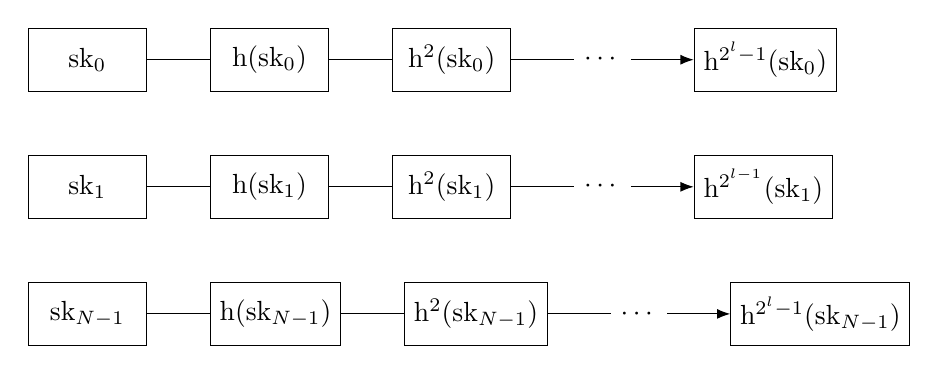
\begin{tikzpicture}[
        node distance=0.8cm and 0.8cm,
        box/.style={
          draw,
          minimum width=1.5cm,
          minimum height=0.8cm,
          align=center
        },
        arr/.style={-{Latex}}
      ]

      % First row: sk_0 → h(sk_0) → h^2(sk_0) → … → h^{2^i−1}(sk_0)
      \node[box] (sk0)    {sk$_0$};
      \node[box,right=of sk0] (hsk0)  {h(sk$_0$)};
      \node[box,right=of hsk0] (h2sk0) {h$^2$(sk$_0$)};
      \node[right=of h2sk0]        (dots0) {$\cdots$};
      \node[box,right=of dots0]  (h2i1sk0) {h$^{2^l-1}$(sk$_0$)};
      \draw[arr] (sk0) -- (hsk0) -- (h2sk0) -- (dots0) -- (h2i1sk0);
    
      % Second row: sk_1 → h(sk_1) → h^2(sk_1) → … → h^{2^i−1}(sk_1)
      \node[box,below=of sk0]    (sk1)    {sk$_1$};
      \node[box,right=of sk1]    (hsk1)   {h(sk$_1$)};
      \node[box,right=of hsk1]   (h2sk1)  {h$^2$(sk$_1$)};
      \node[right=of h2sk1]      (dots1)  {$\cdots$};
      \node[box,right=of dots1] (h2i1sk1){h$^{2^{l-1}}$(sk$_1$)};
      \draw[arr] (sk1) -- (hsk1) -- (h2sk1) -- (dots1) -- (h2i1sk1);
    
      % Last row: sk_{N-1} → h(sk_{N-1}) → h^2(sk_{N-1}) → … → h^{2^i−1}(sk_{N-1})
      \node[box,below=of sk1]    (skN)    {sk$_{N-1}$};
      \node[box,right=of skN]    (hskN)   {h(sk$_{N-1}$)};
      \node[box,right=of hskN]   (h2skN)  {h$^2$(sk$_{N-1}$)};
      \node[right=of h2skN]      (dotsN)  {$\cdots$};
      \node[box,right=of dotsN] (h2i1skN){h$^{2^l-1}$(sk$_{N-1}$)};
      \draw[arr] (skN) -- (hskN) -- (h2skN) -- (dotsN) -- (h2i1skN);
    
        \end{tikzpicture}
            \caption{WOTS key generation}
            \label{fig:WOTS}
        \end{figure}

        In Figure \ref{fig:WOTS}, the secret keys are shown. The public key is obtained by applying the hash function \( 2^l \) times to each secret key (i.e., the \( 2^l \)-th hash). 

        For example, if the value of the first message chunk is 0, then \(\text{sk}_0\) is used in the signature. If the value is \( 2^l - 1 \), then the signature value is \( h^{2^l - 1}(\text{sk}_0) \).

        
    \end{subsubsection}

    \begin{subsubsection}{WOTS Signature}

        For each part of the message, the appropriate number of hash iterations is applied to the corresponding secret key. These hashed values are concatenated to form the complete signature.

        For example, suppose the first three chunks of the message are:
        
        \[
        001 \| 010 \| 111
        \]
        
        Then the first three parts of the signature would be:
        
        \[
        h(\text{sk}_0) \| h^2(\text{sk}_1) \| h^7(\text{sk}_2)
        \]
                
    \end{subsubsection}

    \begin{subsubsection}{WOTS Signature Verification}

        The verifier examines each message part individually. By checking the numerical value of each chunk, the verifier determines how many hash iterations are needed to reach the public key. It then hashes the corresponding part of the signature that many times. The result is compared with the known public key. If all values match, the signature is considered valid.
        
    \end{subsubsection}

    \begin{subsubsection}{WOTS+ \cite{cryptoeprint:2017/965}}

        Introduced as an improved variant of WOTS. The primary difference is that WOTS+ introduces a randomized bitmasking technique in its chaining function. Specifically, before each hash computation in the signature generation and verification process, WOTS+ XORs a randomly generated bitmask with the input. This masking mitigates multi-target attacks and improves the scheme’s resistance to attacks that exploit structural properties of the hash function. 
        
    \end{subsubsection}
    
    
\end{subsection}


\begin{subsection}{Merkle Trees and Multi-Signatures}

Lamport and WOTS schemes are one-time signature algorithms, meaning they allow signing only a single message with generated keys. However, in practical scenarios, signature algorithms are expected to support multiple signatures. To convert one-time signature schemes into algorithms that can sign multiple messages, \textbf{Merkle trees} are used.

As an example, the WOTS scheme can be used together with a Merkle tree. Figure \ref{fig:Merkle} shows the sketch of merkle tree used with WOTS. The bottom leaves of the Merkle tree are the hash values of the WOTS public keys. Using a Merkle tree of height \( h \), a signature scheme capable of signing \( 2^h \) messages can be constructed.

In addition to increasing signature capacity, Merkle trees also have the advantage of \textbf{reducing public key size}. Normally, a WOTS public key consists of multiple components—one for each message chunk—but when used with a Merkle tree, only \textbf{one public key} is required: the root of the Merkle tree.To verify a signature, the verifier must access certain intermediate nodes of the Merkle tree in order to compute the root. These intermediate values can be included as part of the signature, thus enabling successful verification.

\begin{figure}
    \centering
    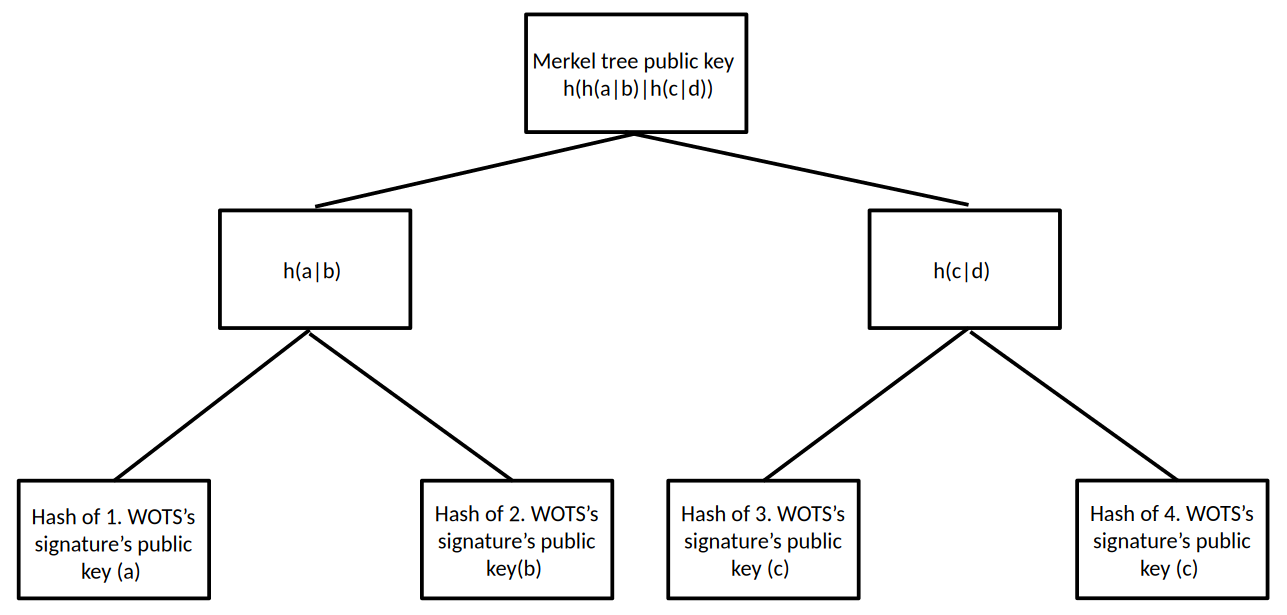
\includegraphics[width=1.1\linewidth]{fig/merkle.png}
    \caption{Merkle Tree}
    \label{fig:Merkle}
\end{figure}

\end{subsection}

\begin{subsection}{L-tree and Hashing public key}{\label{sec:L-tree}}

    When combining one-time signature schemes with a Merkle tree, the public key of the one-time signature scheme is selected as the bottom leaf of the Merkle tree. However, in the WOTS algorithm, a single signature includes not one but multiple public key components—one for each message part.
    
    To resolve this issue, two different approaches are employed:
    
    \begin{enumerate}
        \item \textbf{L-tree (used in XMSS):} The L-tree is a specialized Merkle tree used to compress multiple public key components into a single public key. It repeatedly hashes pairs of public key elements until only one remains.
    
        \item \textbf{Hashing (used in SPHINCS+):} In this method, all public key components are concatenated, and a single hash value is computed over the entire concatenation. This resulting hash serves as the single public key for Merkle tree integration.
    \end{enumerate}

    
\end{subsection}

\begin{subsection}{Base-\texorpdfstring{$w$}{w} Representation }

In hash-based signature schemes such as WOTS and XMSS, the message digest is first transformed into a base-$w$ representation before signing. This \textbf{base-$w$ representation} is a critical component of the signing process and directly influences the structure and security of the signature.

The main purposes of using base-$w$ representation are to:

\begin{itemize}
    \item reduce the size of the signature compared to bit-wise representations (as in the Lamport scheme),
    \item represent the message digest in a form suitable for the Winternitz one-time signature construction,
    \item control the number of hash iterations per key chain in WOTS+,
    \item and balance the trade-off between performance (speed) and signature length through the choice of $w$.
\end{itemize}

Let the output of the hash function be $n$ bits. The number of base-$w$ digits required to represent this $n$-bit message is:
\[
\ell_1 = \left\lceil \frac{8n}{\log_2 w} \right\rceil
\]
Each digit in this representation is an integer in the range $[0, w-1]$, and indicates how many times the corresponding chain of the private key should be hashed to produce the signature component.

\textbf{Example:}  
Suppose $n = 256$ and $w = 16$. Then:
\[
\ell_1 = \left\lceil \frac{8 \cdot 256}{\log_2 16} \right\rceil = \left\lceil \frac{2048}{4} \right\rceil = 512
\]
So, the hash output will be split into 512 base-$16$ digits.

After computing the base-$w$ representation of the message digest, a checksum is computed and appended (as described in the section \ref{sec:Checksum}), forming the complete message input for WOTS+.

The choice of $w$ is significant: 
\begin{itemize}
    \item A smaller $w$ increases the number of digits $\ell_1$ (and thus the signature size) but reduces the number of hash computations.
    \item A larger $w$ reduces the signature size but requires more hash computations per signature, increasing signing and verification time.
\end{itemize}

In summary, the base-$w$ representation enables the WOTS+ signature scheme to efficiently encode the message digest while maintaining flexibility across a range of parameter choices.

\end{subsection}


\begin{subsection}{Checksum}{\label{sec:Checksum}}

In hash-based signature algorithms such as WOTS and XMSS, the message to be signed is first encoded into a base-$w$ representation. However, this encoding alone is not sufficient to ensure security against certain attacks. Therefore, a \textbf{checksum} value is appended to the base-$w$ representation of the message. This checksum serves to:

\begin{itemize}
    \item prevent attacks that attempt to alter message chunks by increasing or decreasing hash iterations,
    \item protect against fault injection attacks that aim to exploit the absence or corruption of the checksum,
    \item and detect message modifications or signature reuse.
\end{itemize}

The checksum is calculated by summing the differences between the maximum possible chunk value $(w-1)$ and each base-$w$ digit of the message. If the message is represented by $m_0, m_1, \ldots, m_{\ell_1-1}$ in base-$w$, the checksum $c$ is given by:
\[
c = \sum_{i=0}^{\ell_1-1} (w - 1 - m_i)
\]
This value is then encoded into base-$w$ as an additional sequence of digits, forming the checksum part of the message. The total number of checksum digits required is $\ell_2$, calculated as:
\[
\ell_2 = \left\lfloor \frac{\log_2(\ell_1(w-1))}{\log_2 w} \right\rfloor + 1
\]

As a result, the full message to be signed by WOTS+ consists of $\ell = \ell_1 + \ell_2$ base-$w$ digits. Each digit corresponds to the number of hash function applications to be performed on a particular chain of the private key.

\textbf{The checksum} plays a crucial role in maintaining the integrity and one-time nature of the WOTS+ signature. Without it, an attacker could transform a valid signature for one message into a valid signature for another message by manipulating the hash chains, which would compromise the existential unforgeability of the scheme.

\end{subsection}


\begin{subsection}{FORS}
    The \textbf{FORS algorithm} (Forest of Random Subsets) is a \textit{few-time signature scheme}. Unlike the WOTS algorithm, in FORS, when the message is divided into parts, a secret key is generated for each possible value of every part, and a small Merkle tree is constructed from these keys.
    The signature consists of:
    \begin{itemize}
        \item The secret key corresponding to the integer value of the message part.
        \item The necessary authentication path (intermediate nodes) to reach the root of the Merkle tree.
    \end{itemize}
    An example FORS signature for the below message is shown in Figure \ref{fig:FORS}.
    
    \[100 \quad 011 \quad 011 \quad 101 \quad 111 \quad 000\]
    
    
    \begin{figure}
        \centering
        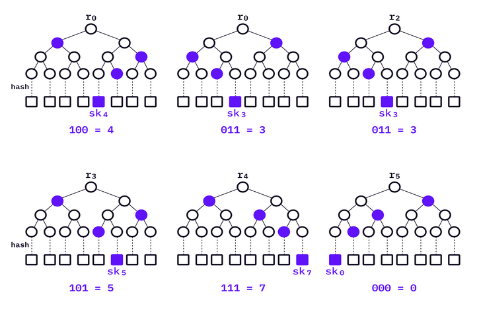
\includegraphics[width=0.9\linewidth]{fig/FORS.png}
        \caption{FORS Signature example }
        \label{fig:FORS}
    \end{figure}

\end{subsection}

\begin{subsection}{Address Structures in Hash-Based Signature Schemes}
    Hash-based signature schemes consist of either very large Merkle trees or multi-layered Merkle trees in order to increase their signature capacity. Since the same hash function is repeatedly used within the tree and similar operations are performed, \textbf{address structures} are used in hash-based signature schemes to:
\begin{itemize}
    \item distinguish each operation,
    \item determine the position within the tree,
    \item track how many hash operations have been applied,
    \item and provide input differentiation for the hash functions.
\end{itemize}

\textbf{Table} \ref{tab: Adress} shows the \textbf{OTS address structure} used in the XMSS algorithm \cite{huelsing2018rfc}. In the example structure, the following fields appear in order from top to bottom:
\begin{itemize}
    \item the layer in the multi-tree,
    \item the specific tree identifier,
    \item address type (e.g., OTS),
    \item index of the L-tree–WOTS pair,
    \item WOTS chain identifier,
    \item index of the hash operation within the chain,
    \item a flag indicating whether the hash value is used for encryption or masking.
\end{itemize}

Depending on the algorithm and its internal structure, the format of the address field can vary.


\begin{table}[H]
\centering
\renewcommand{\arraystretch}{1.5}
\begin{tabular}{|c|c|}
\hline
\textbf{Field} & \textbf{Size} \\
\hline
layer address     & 32 bits \\
\hline
tree address      & 64 bits \\
\hline
type = 0          & 32 bits \\
\hline
OTS address       & 32 bits \\
\hline
chain address     & 32 bits \\
\hline
hash address      & 32 bits \\
\hline
keyAndMask        & 32 bits \\
\hline
\end{tabular}
\caption{XMSS OTS Address Format}
\label{tab: Adress}
\end{table}

\end{subsection}

\begin{subsection}{Stateful and Stateless Hash-Based Signature Schemes}

    Hash-based signature algorithms can be categorized into two types: \textbf{stateful} and \textbf{stateless}. The fundamental difference between these two categories lies in the management of state information during the signature generation and verification processes.

\textbf{Stateful hash-based signature algorithms} require the maintenance of state information while generating signatures. These algorithms rely on \textit{one-time keys} that can be used only once per signature operation. Reusing these keys leads to serious security vulnerabilities. A representative example of such an algorithm is XMSS \cite{huelsing2018rfc}.

\textbf{Stateless hash-based signature algorithms}, in contrast, do not require any state information to be stored during the signing process. A prominent example of a stateless algorithm is SPHINCS+ \cite{bernstein2019sphincs+}.
    
\end{subsection}

\end{section}
\begin{section}{XMSS and $XMSS^{MT}$}

    In this section, the XMSS/$XMSS^{MT}$ algorithms, as defined in the documents \cite{cooper2020recommendation} \cite{huelsing2018rfc} , will be explained using the fundamental structures presented in Section \ref{sec1}. Arhitecrure of the XMSS is given in the Figure \ref{fig:xmss}

\begin{figure}[h]
\centering
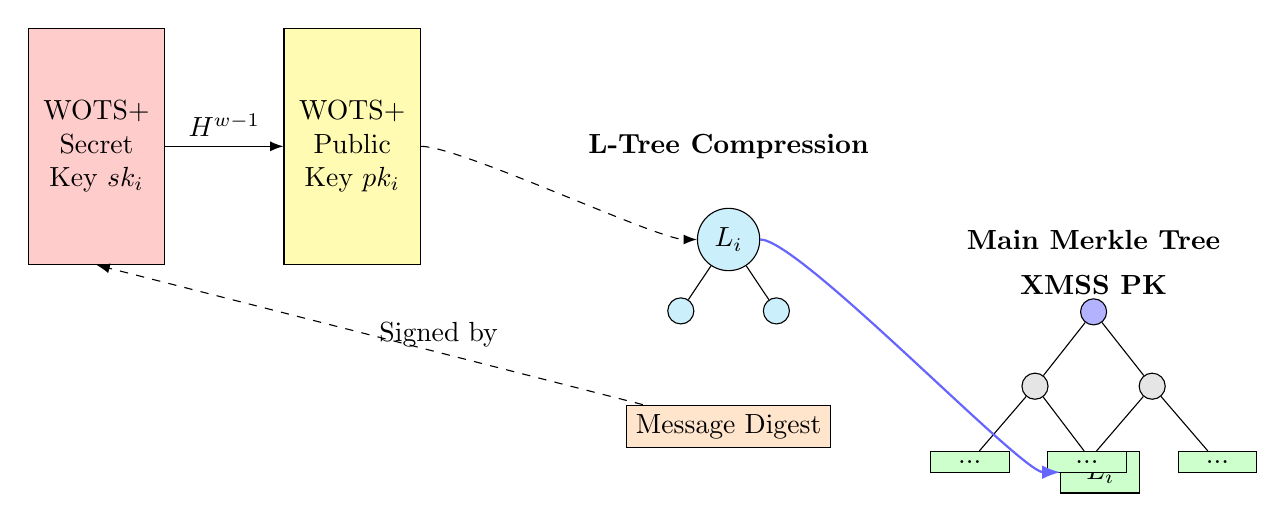
\begin{tikzpicture}[
    node distance=1.5cm,
    wots_pk/.style={rectangle, draw, fill=yellow!30, text width=1.5cm, align=center, minimum height=3cm},
    wots_sk/.style={rectangle, draw, fill=red!20, text width=1.5cm, align=center, minimum height=3cm},
    ltree_node/.style={circle, draw, fill=cyan!20},
    merkle_node/.style={circle, draw, fill=gray!20},
    leaf_node/.style={rectangle, draw, fill=green!20, minimum width=1cm},
    main_root/.style={merkle_node, fill=blue!30, label={[label distance=-2pt]90:\textbf{XMSS PK}}}
]

% WOTS+ Part
\node[wots_sk] (wots_sk) {WOTS+ Secret Key $sk_i$};
\node[wots_pk, right=of wots_sk] (wots_pk) {WOTS+ Public Key $pk_i$};
\draw[-Latex] (wots_sk) -- (wots_pk) node[midway, above] {$H^{w-1}$};

% L-Tree Part
\node[right=2cm of wots_pk] (ltree_label) {\textbf{L-Tree Compression}};
\node[ltree_node, below=0.5cm of ltree_label] (ltree_root) {$L_i$};
\node[ltree_node, below left=0.5cm and 0.2cm of ltree_root] (ltree1) {};
\node[ltree_node, below right=0.5cm and 0.2cm of ltree_root] (ltree2) {};
\draw (ltree1) -- (ltree_root) -- (ltree2);
\draw[-Latex, dashed] (wots_pk.east) .. controls +(0.5,0) and +(-0.5,0) .. (ltree_root.west);

% Merkle Tree Part
\node[right=2.5cm of ltree_root] (mt_label) {\textbf{Main Merkle Tree}};
\node[main_root, below=0.5cm of mt_label] (root) {};
\node[merkle_node, below left=0.7cm and 0.5cm of root] (n1) {};
\node[merkle_node, below right=0.7cm and 0.5cm of root] (n2) {};
\node[leaf_node, below left=0.7cm and 0.2cm of n1] (L0) {...};
\node[leaf_node, below right=0.7cm and 0.2cm of n1] (Li) {$L_i$};
\node[leaf_node, below left=0.7cm and 0.2cm of n2] (Lj) {...};
\node[leaf_node, below right=0.7cm and 0.2cm of n2] (LN) {...};
\draw (root) -- (n1) -- (L0);
\draw (n1) -- (Li);
\draw (root) -- (n2) -- (Lj);
\draw (n2) -- (LN);

% Connection from L-Tree to Merkle Tree
\draw[-Latex, thick, blue!60] (ltree_root.east) .. controls +(0.5,0) and +(-0.5,0) .. (Li.west);

% Signing part
\node[rectangle, draw, fill=orange!20, below=3cm of ltree_label] (msg) {Message Digest};
\draw[-Latex, dashed] (msg) -- (wots_sk.south) node[midway, right, text width=2cm] {Signed by};

\end{tikzpicture}
\caption{The architecture of XMSS. A WOTS+ key pair signs a message. Its public key is compressed via an L-Tree into a single leaf $L_i$. This leaf is part of a large Merkle tree, whose root serves as the overall XMSS public key.}
\label{fig:xmss}
\end{figure}


    \begin{subsection}{XMSS Key Generation}

        In Algorithm \ref{alg:XMSS_keygen}, a pseudo-code representation of the key generation process of the \textbf{XMSS} algorithm is provided. First, the \textbf{WOTS} private keys are generated. These keys can be created either completely at random or by passing a seed value through a key generation function. If all keys are generated randomly, they must be stored in memory for the signing process. However, since storing all the keys in memory is not realistic, this method is generally not used. Next, certain seed values are generated to be used throughout the algorithm, and the hash values of the WOTS private keys are taken to produce the WOTS public keys. In the pseudo-code, the value \texttt{idx} at the beginning of the \texttt{SK} section represents the state information.

        \begin{algorithm}
\caption{XMSS\_keyGen -- Generate an XMSS key pair}
\label{alg:XMSS_keygen}

\textbf{Input:} None \\
\textbf{Output:} XMSS private key \texttt{SK}, XMSS public key \texttt{PK}

\vspace{0.3cm}

\begin{tabular}{ll}
1: & \textit{// Example initialization for SK-specific contents} \\
2: & \texttt{idx} $\leftarrow 0$ \\
3: & \textbf{for} $i = 0$ \textbf{to} $2^h - 1$ \textbf{do} \\
4: & \quad \texttt{wots\_sk[i]} $\leftarrow$ \texttt{WOTS\_genSK()} \\
5: & \textbf{end for} \\
6: & Initialize \texttt{SK\_PRF} with a uniformly random $n$-byte string \\
7: & \texttt{setSK\_PRF(SK, SK\_PRF)} \\
8: & \textit{// Initialization for common contents} \\
9: & Initialize \texttt{SEED} with a uniformly random $n$-byte string \\
10: & \texttt{setSEED(SK, SEED)} \\
11: & \texttt{setWOTS\_SK(SK, wots\_sk)} \\
12: & \texttt{ADRS} $\leftarrow$ \texttt{toByte(0, 32)} \\
13: & \texttt{root} $\leftarrow$ \texttt{treeHash(SK, 0, h, ADRS)} \\
14: & \texttt{SK} $\leftarrow$ \texttt{idx $\parallel$ wots\_sk $\parallel$ SK\_PRF $\parallel$ root $\parallel$ SEED} \\
15: & \texttt{PK} $\leftarrow$ \texttt{OID $\parallel$ root $\parallel$ SEED} \\
16: & \textbf{return} \texttt{SK $\parallel$ PK}
\end{tabular}

\end{algorithm}

        
    \end{subsection}

    \begin{subsection}{XMSS Sign}

        In Algorithm \ref{alg:XMSS_sign}, the pseudo-code of the XMSS signing algorithm is presented. The \texttt{treeSig} function signs the message using WOTS and generates the authentication path required to reach the root of the tree. First, the state information is retrieved, then a random value is generated and concatenated with the message, after which a hash is computed from this combination. This hash value is then signed using the \texttt{treeSig} algorithm. The final signature consists of the concatenation of the state information, the random value, and the \texttt{treeSig} signature, respectively.


        \begin{algorithm}
\caption{XMSS\_sign – Generate an XMSS signature and update the XMSS private key}
\label{alg:XMSS_sign}

\textbf{Input:} Message $M$, XMSS private key $SK$ \\
\textbf{Output:} Updated $SK$, XMSS signature $Sig$

\vspace{0.3cm}

\begin{tabular}{ll}
1: & \texttt{idx\_sig} $\leftarrow$ \texttt{getIdx(SK)} \\
2: & \texttt{setIdx(SK, idx\_sig + 1)} \\
3: & \texttt{ADRS} $\leftarrow$ \texttt{toByte(0, 32)} \\
4: & \texttt{r} $\leftarrow$ \texttt{PRF(getSK\_PRF(SK), toByte(idx\_sig, 32))} \\
5: & \texttt{M'} $\leftarrow$ \texttt{H\_msg(r $\parallel$ getRoot(SK) $\parallel$ toByte(idx\_sig, n), M)} \\
6: & \texttt{Sig} $\leftarrow$ \texttt{idx\_sig $\parallel$ r $\parallel$ treeSig(M', SK, idx\_sig, ADRS)} \\
7: & \textbf{return} \texttt{SK $\parallel$ Sig}
\end{tabular}

\end{algorithm}

        
\end{subsection}

\begin{subsection}{XMSS Verify}

In Algorithm \ref{alg:xmss_rootfromSign} and \ref{alg:xmss_verify}, the pseudo-code of the XMSS signature verification is presented. First, the WOTS public key is derived from the message. Then, these WOTS public keys are passed through the \texttt{L-tree} to obtain the leaves of the Merkle tree. From the leaves of the Merkle tree, the root is reached to obtain the XMSS public key and perform verification. If the derived public key matches the expected value, the signature is considered valid. The authentication path contained in the signature is used to climb to the root in both the \texttt{L-tree} and the Merkle tree.

\begin{algorithm}
\caption{XMSS\_rootFromSig: Compute a root node from a tree signature}
\label{alg:xmss_rootfromSign}

\textbf{Input:} \\
\quad index \texttt{idx\_sig} \\
\quad WOTS+ signature \texttt{sig\_ots} \\
\quad authentication path \texttt{auth} \\
\quad $n$-byte message $M'$ \\
\quad seed \texttt{SEED} \\
\quad address \texttt{ADRS} \\[0.2cm]
\textbf{Output:} $n$-byte root value \texttt{node[0]}

\vspace{0.3cm}

\begin{tabular}{ll}
1: & \texttt{ADRS.setType(0)} \hfill \textit{// Type = OTS hash address} \\
2: & \texttt{ADRS.setOTSAddress(idx\_sig)} \\
3: & \texttt{pk\_ots} $\leftarrow$ \texttt{WOTS\_pkFromSig(sig\_ots, M', SEED, ADRS)} \\
4: & \texttt{ADRS.setType(1)} \hfill \textit{// Type = L-tree address} \\
5: & \texttt{ADRS.setLTreeAddress(idx\_sig)} \\
6: & Initialize \texttt{node[0]} and \texttt{node[1]} as $n$-byte arrays \\
7: & \texttt{node[0]} $\leftarrow$ \texttt{ltree(pk\_ots, SEED, ADRS)} \\
8: & \texttt{ADRS.setType(2)} \hfill \textit{// Type = hash tree address} \\
9: & \texttt{ADRS.setTreeIndex(idx\_sig)} \\
10: & \textbf{for} $k = 0$ \textbf{to} $h-1$ \textbf{do} \\
11: & \quad \texttt{ADRS.setTreeHeight(k)} \\
12: & \quad \textbf{if} $\left\lfloor \texttt{idx\_sig} / 2^k \right\rfloor \bmod 2 = 0$ \textbf{then} \\
13: & \qquad \texttt{ADRS.setTreeIndex(ADRS.getTreeIndex() / 2)} \\
14: & \qquad \texttt{node[1]} $\leftarrow$ \texttt{RAND\_HASH(node[0], auth[k], SEED, ADRS)} \\
15: & \quad \textbf{else} \\
16: & \qquad \texttt{ADRS.setTreeIndex((ADRS.getTreeIndex() - 1) / 2)} \\
17: & \qquad \texttt{node[1]} $\leftarrow$ \texttt{RAND\_HASH(auth[k], node[0], SEED, ADRS)} \\
18: & \quad \textbf{end if} \\
19: & \quad \texttt{node[0]} $\leftarrow$ \texttt{node[1]} \hfill \textit{// Update current node} \\
20: & \textbf{end for} \\
21: & \textbf{return} \texttt{node[0]}
\end{tabular}

\end{algorithm}


        \begin{algorithm}
        \caption{XMSS\_verify -- Verify an XMSS signature using the corresponding XMSS public key and a message}
        \label{alg:xmss_verify}
        \textbf{Input:} XMSS signature \texttt{Sig}, message \texttt{M}, XMSS public key \texttt{PK} \\
        \textbf{Output:} Boolean
        
        \vspace{0.2cm}
        
        \begin{tabular}{ll}
        1: & \texttt{ADRS} $\leftarrow$ \texttt{toByte(0, 32)} \\
        2: & \texttt{M'} $\leftarrow$ \texttt{H\_msg(r || getRoot(PK) || toByte(idx\_sig, n), M)} \\
        3: & \texttt{node} $\leftarrow$ \texttt{XMSS\_rootFromSig(idx\_sig, sig\_ots, auth, M', getSEED(PK), ADRS)} \\
        4: & \textbf{if} \texttt{node == getRoot(PK)} \textbf{then} \\
        5: & \hspace{0.5cm} \textbf{return} \texttt{true} \\
        6: & \textbf{else} \\
        7: & \hspace{0.5cm} \textbf{return} \texttt{false} \\
        8: & \textbf{end if}
        \end{tabular}
        
        \end{algorithm}
        
    \end{subsection}

    \begin{subsection}{$XMSS^{MT}$}
        $XMSS^{MT}$ is the multi-tree version of the XMSS algorithm. While the XMSS algorithm consists of a single large tree, the multi-tree structure comprises many smaller trees, each signing the public key of the next. The advantage of this approach is that signing is faster because it eliminates the need to generate the entire large tree during the signature verification process. In a multi-tree structure, the signature is formed by the combination of the signatures and authentication paths of each layer. Figure \ref{fig:MTsig} shows the multi-tree signature structure. Figure \ref{fig:MTstruc} illustrates the overall structure of the multi-tree.

        


        \begin{figure}
        \centering
        \begin{subfigure}{0.5\textwidth}
          \centering
          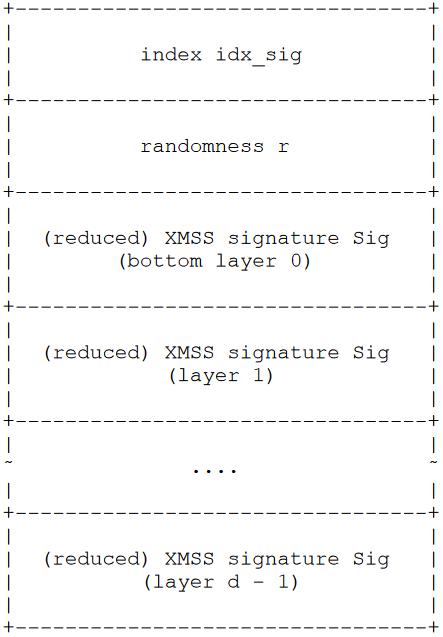
\includegraphics[width=\linewidth]{fig/MTsignature.png}
          \caption{Multi-tree signature}
          \label{fig:MTsig}
          
        \end{subfigure}%
        \begin{subfigure}{0.5\textwidth}
          \centering
          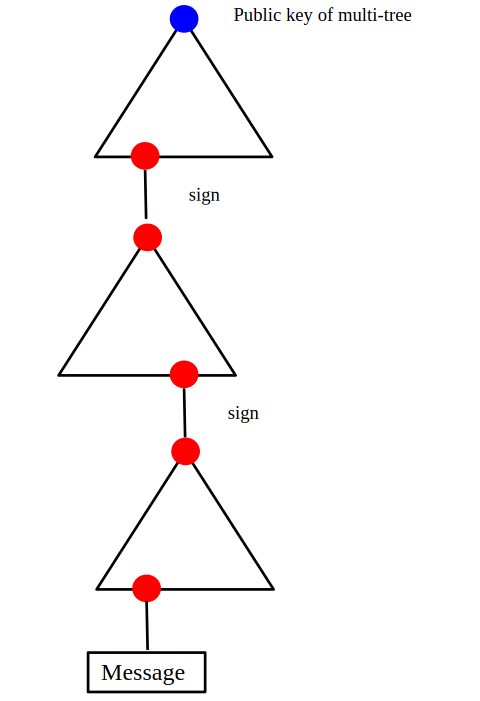
\includegraphics[width=\linewidth]{fig/multi-tree.png}
          \caption{Multi-tree general structure}
          \label{fig:MTstruc}
          
        \end{subfigure}
        \caption{XMSS multi-tree}
        \label{fig:LAT}
        \end{figure}


        
    \end{subsection}

    
    
\end{section}
\begin{section}{SPHINCS+}

    SPHINCS+ \cite{gaithersburgmdnist_2024_stateless} is one of the three signature algorithms standardized by NIST. Structurally, it is very similar to XMSS. Fundamentally, there are two main differences. First, the SPHINCS+ algorithm does not use an L-tree structure. Instead, it transforms WOTS public keys into a single public key by applying a hash function.(see section \ref{sec:L-tree}) Second, unlike XMSS, which contains only a WOTS signature, the SPHINCS+ algorithm also includes a FORS signature layer underneath the WOTS signature. Since the FORS signature algorithm is not a one-time signature, it allows multiple signatures to be generated from the same tree. For this reason, SPHINCS+ is a stateless algorithm. Before each signing operation, it selects a random index and generates the signature and authentication path from the part of the tree corresponding to that index. Because it does not require securely storing and updating state information, stateless SPHINCS+ offers a significant advantage over XMSS in this regard. However, the FORS layer, which makes SPHINCS+ stateless, adds an additional layer of signature under WOTS, thereby increasing the signature size compared to XMSS. Due to the tree-based structure of hash-based signature algorithms, both algorithms have the same public key size. Figure \ref{fig:SPHINCS} illustrates the general structure of the SPHINCS+ algorithm. 
    \begin{subsection}{SPHINCS+ Parameters}
        Parameters and their descriptions are given below: 
    \begin{description}
  \item[$n$:] Hash output size in bits. All outputs of the underlying hash functions (e.g., $H_{\mathrm{msg}}$, PRF, and Merkle-node hashes) are exactly $n$ bits long.
  
  \item[$w$:] Winternitz parameter. Determines the base for WOTS\texttt{+} chains.  
    Higher $w$ reduces signature length at the cost of more hash computations per chain.

  \item[$\ell$:] Total number of $n$-bit chains in each WOTS\texttt{+} key or signature, given by


\[
    \ell = \ell_1 + \ell_2,
    \quad
    \ell_1 = \left\lceil \frac{8n}{\log_2 w} \right\rceil,
    \quad
    \ell_2 = \left\lfloor \frac{\log_2(\ell_1\,(w-1))}{\log_2 w} \right\rfloor + 1.
  \]

  \item[$h$:] Total height of the Merkle hypertree.  
    The overall number of leaves (XMSS key pairs) is $2^h$.

  \item[$h'$:] Height of each XMSS subtree.  
    Each subtree contains $2^{h'}$ leaves, and we arrange $d$ such layers to reach height $h$.

  \item[$d$:] Number of layers in the hypertree, satisfying
  
\[
    d = \frac{h}{h'}.
  \]

  \item[$k$:] Number of parallel FORS trees.  
    The $n$-bit message digest is split into $k$ indices, each signed by one FORS tree.
\end{description}
    \end{subsection}
    


    \begin{figure}[H]
        \centering
        % Private Key Table
        \begin{minipage}{0.45\textwidth}
        \centering
        \begin{tabular}{|l|l|}
        \hline
        \textbf{SK.seed} & $n$ bytes \\
        \hline
        \textbf{SK.prf}  & $n$ bytes \\
        \hline
        \textbf{PK.seed} & $n$ bytes \\
        \hline
        \textbf{PK.root} & $n$ bytes \\
        \hline
        \end{tabular}
        \caption{SPHINCS+ private key}
        \label{fig:slhdsa_privatekey}
        \end{minipage}
        \hfill
        % Public Key Table
        \begin{minipage}{0.45\textwidth}
        \centering
        \begin{tabular}{|l|l|}
        \hline
        \textbf{PK.seed} & $n$ bytes \\
        \hline
        \textbf{PK.root} & $n$ bytes \\
        \hline
        \end{tabular}
        \caption{SPHINCS+ public key}
        \label{fig:slhdsa_publickey}
        \end{minipage}
        
    \end{figure}


    \begin{figure}
        \centering
        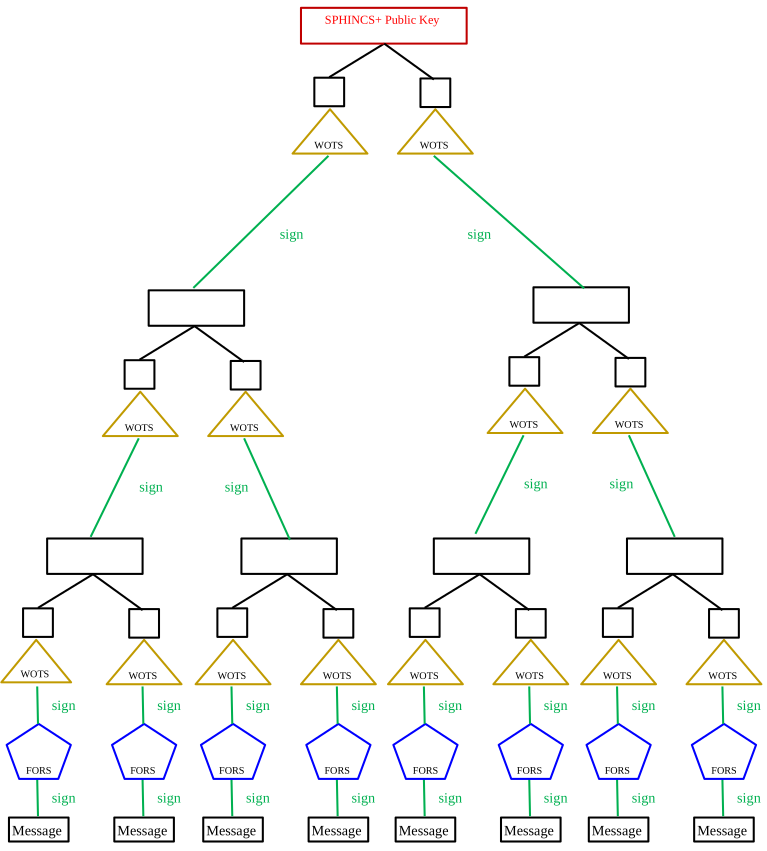
\includegraphics[width=1.1\linewidth]{fig/sphıncs.png}
        \caption{SPHINCS+ General structure}
        \label{fig:SPHINCS}
    \end{figure}
\end{section}


\begin{subsection}{SPHINCS+ Key Generation}

Key generation derives a full SPHINCS+ key pair from three seeds: the secret seed, the PRF key, and the public seed. It first initializes the ADRS value with a zero‐filled 32‐byte string and configures it for the top-level XMSS tree by setting the layer address to \(d-1\). The root node of that tree is computed via a single call to \texttt{xmss\_node}, which absorbs the secret seed, the public seed, and the ADRS state. Finally, the algorithm returns the secret key tuple \((\mathit{SK}.\mathit{seed},\,\mathit{SK}.\mathit{prf},\,\mathit{PK}.\mathit{seed},\,\mathit{PK}.\mathit{root})\) alongside the public key \((\mathit{PK}.\mathit{seed},\,\mathit{PK}.\mathit{root})\) (see Algorithm~\ref{alg:sphincs_keygen}).

\begin{algorithm}
\caption{SPHINCS\_keyGen -- Generate a SPHINCS+ key pair}
\label{alg:sphincs_keygen}

\textbf{Input:} None \\
\textbf{Output:} SPHINCS+ private key \texttt{SK}, SPHINCS+ public key \texttt{PK}

\vspace{0.3cm}

\begin{tabular}{ll}
1: & Generate uniformly random $n$-byte strings: \texttt{SK.SEED}, \texttt{SK.PRF}, \texttt{PK.SEED} \\
2: & Initialize \texttt{ADRS} as a zeroed address structure \\
3: & \texttt{PK.root} $\leftarrow$ \texttt{treehash(SK\_SEED, PUB\_SEED, ADRS)} \\
4: & \texttt{SK} $\leftarrow$ \texttt{SK.SEED $\parallel$ SK.PRF $\parallel$ PUB.SEED $\parallel$ PK.root} \\
5: & \texttt{PK} $\leftarrow$ \texttt{PK.SEED $\parallel$ PK.root} \\
6: & \textbf{return} \texttt{SK, PK}
\end{tabular}
\end{algorithm}

\end{subsection}

\begin{subsection}{SPHINCS+ Sign}

Signature generation begins by initializing the ADRS to zero and optionally randomizing the message randomizer input. The PRF keyed by \(\mathit{SK}.\mathit{prf}\) produces the randomness \(R\) that is prepended to the signature. A message digest is then computed over \(R\), the public seed, the root, and the message itself. This digest is split into the message digest bits \(\mathit{md}\) and the tree/leaf indices \(\mathit{idx\_tree},\mathit{idx\_leaf}\). The FORS scheme is applied at the lowest layer (layer 0) to sign \(\mathit{md}\), yielding \(\mathit{SIG\_FORS}\) and an authenticated public key \(\mathit{PK\_FORS}\). Finally, the hypertree (HT) signature over \(\mathit{PK\_FORS}\) is computed and appended, producing the full SPHINCS+ signature (see Algorithm~\ref{alg:spx_sign})

\begin{algorithm}
    \caption{spx\_sign -- Generating a SPHINCS+ signature}
    \label{alg:spx_sign}
    \textbf{Input:} Message \texttt{M}, private key \texttt{SK} = (\texttt{SK.seed}, \texttt{SK.prf}, \texttt{PK.seed}, \texttt{PK.root}) \\
    \textbf{Output:} SPHINCS+ signature \texttt{SIG}

    \vspace{0.2cm}

    \begin{tabular}{ll}
    1:  & \texttt{ADRS} $\leftarrow$ \texttt{toByte(0, 32)} \\
    2:  & \texttt{opt}  $\leftarrow$ \texttt{PK.seed} \\
    3:  & \textbf{if} \texttt{RANDOMIZE} \textbf{then} \\
    4:  & \quad \texttt{opt}  $\leftarrow$ \texttt{rand(n)} \\
    5:  & \textbf{end if} \\
    6:  & \texttt{R}    $\leftarrow$ \texttt{PRF\_msg(SK.prf, opt, M)} \\
    7:  & \texttt{SIG}  $\leftarrow$ \texttt{R} \\
    8:  & \texttt{digest} $\leftarrow$ \texttt{H\_msg(R, PK.seed, PK.root, M)} \\
    9:  & \texttt{tmp\_md}       $\leftarrow$ first $\lfloor(\mathit{ka}+7)/8\rfloor$ bytes of \texttt{digest} \\
    10: & \texttt{tmp\_idx\_tree} $\leftarrow$ next $\lfloor(h - h/d +7)/8\rfloor$ bytes of \texttt{digest} \\
    11: & \texttt{tmp\_idx\_leaf} $\leftarrow$ next $\lfloor(h/d +7)/8\rfloor$ bytes of \texttt{digest} \\
    12: & \texttt{md}      $\leftarrow$ first \texttt{ka} bits of \texttt{tmp\_md} \\
    13: & \texttt{idx\_tree} $\leftarrow$ first $(h - h/d)$ bits of \texttt{tmp\_idx\_tree} \\
    14: & \texttt{idx\_leaf} $\leftarrow$ first $h/d$ bits of \texttt{tmp\_idx\_leaf} \\
    15: & \texttt{ADRS.setLayerAddress(0)} \\
    16: & \texttt{ADRS.setTreeAddress(idx\_tree)} \\
    17: & \texttt{ADRS.setType(FORS\_TREE)} \\
    18: & \texttt{ADRS.setKeyPairAddress(idx\_leaf)} \\
    19: & \texttt{SIG\_FORS} $\leftarrow$ \texttt{fors\_sign(md, SK.seed, PK.seed, ADRS)} \\
    20: & \texttt{SIG}      $\leftarrow$ \texttt{SIG} \texttt{||} \texttt{SIG\_FORS} \\
    21: & \texttt{PK\_FORS} $\leftarrow$ \texttt{fors\_pkFromSig(SIG\_FORS, md, PK.seed, ADRS)} \\
    22: & \texttt{ADRS.setType(TREE)} \\
    23: & \texttt{SIG\_HT}   $\leftarrow$ \texttt{ht\_sign(PK\_FORS, SK.seed, PK.seed, idx\_tree, idx\_leaf)} \\
    24: & \texttt{SIG}      $\leftarrow$ \texttt{SIG} \texttt{||} \texttt{SIG\_HT} \\
    25: & \textbf{return} \texttt{SIG}
    \end{tabular}
\end{algorithm}



\begin{table}[ht]
  \centering
  \begin{tabular}{|l|}
    \hline
    \textbf{Signature}                         \\ \hline
    Randomness \(R\)                         \\ \hline
    FORS Signature \(\mathrm{SIG}_{\mathrm{FORS}}\)        \\ \hline
    HT Signature \(\mathrm{SIG}_{\mathrm{HT}}\)        \\ \hline
  \end{tabular}
  \caption{SPHINCS+ signature data format}
  \label{tab:slh-dsa-format}
\end{table}



\end{subsection}

\begin{subsection}{SPHINCS+ Verify}

Verification mirrors signing: it parses the incoming signature into \(R\), \(\mathit{SIG\_FORS}\), and \(\mathit{SIG\_HT}\). The verifier recomputes the message digest and splits it into \(\mathit{md}\), \(\mathit{idx\_tree}\), and \(\mathit{idx\_leaf}\). It then re-derives the FORS public key by running \(\mathit{fors\_pkFromSig}\) on \(\mathit{SIG\_FORS}\) and \(\mathit{md}\). Finally, the hypertree signature is checked with \(\mathit{ht\_verify}\), which returns \(\mathit{true}\) only if every component matches the stored public root (see Algorithm~\ref{alg:spx_verify}).

\begin{algorithm}
    \caption{spx\_verify -- Verify a SPHINCS+ signature SIG on a message M using a SPHINCS+ public key PK}
    \label{alg:spx_verify}
    \textbf{Input:} Message \texttt{M}, signature \texttt{SIG}, public key \texttt{PK} \\
    \textbf{Output:} Boolean

    \vspace{0.2cm}

    \begin{tabular}{ll}
        1:  & \texttt{ADRS} $\leftarrow$ \texttt{toByte(0, 32)} \\
        2:  & \texttt{R} $\leftarrow$ \texttt{SIG.getR()} \\
        3:  & \texttt{SIG\_FORS} $\leftarrow$ \texttt{SIG.getSIG\_FORS()} \\
        4:  & \texttt{SIG\_HT} $\leftarrow$ \texttt{SIG.getSIG\_HT()} \\
        5:  & \texttt{digest} $\leftarrow$ \texttt{H\_msg(R, PK.seed, PK.root, M)} \\
        6:  & \texttt{tmp\_md} $\leftarrow$ first $\lfloor(\mathit{ka}+7)/8\rfloor$ bytes of \texttt{digest} \\
        7:  & \texttt{tmp\_idx\_tree} $\leftarrow$ next $\lfloor(h - h/d +7)/8\rfloor$ bytes of \texttt{digest} \\
        8:  & \texttt{tmp\_idx\_leaf} $\leftarrow$ next $\lfloor(h/d +7)/8\rfloor$ bytes of \texttt{digest} \\
        9:  & \texttt{md} $\leftarrow$ first \texttt{ka} bits of \texttt{tmp\_md} \\
        10: & \texttt{idx\_tree} $\leftarrow$ first $(h - h/d)$ bits of \texttt{tmp\_idx\_tree} \\
        11: & \texttt{idx\_leaf} $\leftarrow$ first $h/d$ bits of \texttt{tmp\_idx\_leaf} \\
        12: & \texttt{ADRS.setLayerAddress(0)} \\
        13: & \texttt{ADRS.setTreeAddress(idx\_tree)} \\
        14: & \texttt{ADRS.setType(FORS\_TREE)} \\
        15: & \texttt{ADRS.setKeyPairAddress(idx\_leaf)} \\
        16: & \texttt{PK\_FORS} $\leftarrow$ \texttt{fors\_pkFromSig(SIG\_FORS, md, PK.seed, ADRS)} \\
        17: & \texttt{ADRS.setType(TREE)} \\
        18: & \textbf{return} \texttt{ht\_verify(PK\_FORS, SIG\_HT, PK.seed, idx\_tree, idx\_leaf, PK.root)} \\
    \end{tabular}
\end{algorithm}


\end{subsection}

\newpage
\begin{section}{Some Attacks on Hash Based Signatures}


This section examines some attacks on hash-based signature algorithms.

\subsection{Intermediate Value Guessing Attack}

This attack was defined in the paper by Booth et al.\cite{booth2021intermediate}. In the document by Hülsing et al. \cite{huelsing2018rfc}, it is stated that the secret key values used in the WOTS+ signature must be generated in a uniformly distributed , but the method is left to the implementer. Assume that the WOTS+ secret keys (\texttt{osk}) are generated from the seed values \texttt{seed\textsubscript{OTS},i} as follows:

\[
\texttt{osk} = (x_{i,1}, x_{i,2}, \ldots, x_{i,l}) = (F(\texttt{seed}_{\text{OTS},i},1), \ldots, F(\texttt{seed}_{\text{OTS},i},l))
\]

Under this assumption:

\begin{itemize}
    \item The signatures of messages whose base-$w$ representation includes zero values leak the corresponding indices of \texttt{osk}. For instance, if the base-$w$ representation of message $M$ is $BM = (b_1, 0, b_2)$, then the signature $\sigma_M = (Z_1, x_{i,2}, Z_3)$ reveals $x_{i,2}$. (Here, each $Z$ value is derived by applying the hash algorithm to a secret key index $w$ times.)
    
    \item The \texttt{osk} values used to sign different messages are generated from different seed values.
    
    \item Using a different seed for each WOTS+ secret key allows a multi-target attack, as described below.
\end{itemize}

In this attack, the adversary proceeds as follows:

\begin{itemize}
    \item Executes the signing oracle to obtain multiple WOTS+ message-signature pairs.
    \item Filters out pairs where fewer than two \texttt{osk} values are revealed.
    \item Assumes that a signature has the form $\sigma = (Z_1, \ldots, Z_l)$ and the message base-$w$ representation is $BM = (b_1, \ldots, b_l)$. The adversary identifies two indices $k_1$ and $k_2$ such that $Z_1$ and $Z_2$ correspond to $x_{i,k_1}$ and $x_{i,k_2}$ respectively. (Here, $k_1$ and $k_2$ are the positions where the base-$w$ value is zero.)
    
    \item From this, the adversary learns:
    \[
    x_{i,k_1} = F(\texttt{seed}_{\text{OTS},i}, k_1), \quad x_{i,k_2} = F(\texttt{seed}_{\text{OTS},i}, k_2)
    \]
    
    \item Using these values, the adversary constructs tables from message-signature pairs (assuming layer $j$ is known):
    \[
    (x_{k_1,k_2}, x_{k_2,i}, j), \quad (x_{k_3,k_4}, x_{k_4,i}, j)
    \]
    
    \item For each guessed \texttt{seed\textsubscript{OTS},i}, the adversary reconstructs a candidate $\texttt{osk}'$ and checks whether the generated value matches existing entries in the table. If both $x_{k_1}$ and $x_{k_2}$ match, the guess for $\texttt{seed\textsubscript{OTS},i}$ is considered correct.
\end{itemize}

Assuming the adversary correctly guesses $\texttt{seed}_{\text{OTS},i}$, let the message $M_i$ have the following XMSSMT signature structure. To forge a valid signature, the adversary uses one of the following strategies:

\paragraph{Case 1: Seed Belongs to Layer 0}

At layer 0, the signature is generated by signing $H(R \,\|\, \texttt{ROOT} \,\|\, i, M_i)$. Let $M_j$ be the adversary’s chosen message. The adversary computes $H(R \,\|\, \texttt{ROOT} \,\|\, i, M_j)$, signs it with the recovered secret key, and replaces the original signature value with this forged one. The authentication path values (\texttt{Auth}) remain unchanged, as they depend on the secret key used, not the signed message.

\paragraph{Case 2: Seed Belongs to Layer $j > 0$}

Suppose the recovered seed belongs to a WOTS+ instance at layer $j > 0$. In this case, the WOTS+ signs the root of layer $j-1$. In XMSSMT, signature verification is performed by computing the root at each layer and comparing the top-layer root with the public key. If the seed belongs to a layer $j > 0$, the adversary can forge the subtree below layer $j$ for a chosen message, replacing the signature value at layer $j$ while keeping the rest of the signature unchanged. Since the upper layers remain valid, the signature is accepted as legitimate.

\begin{figure}
    \centering
    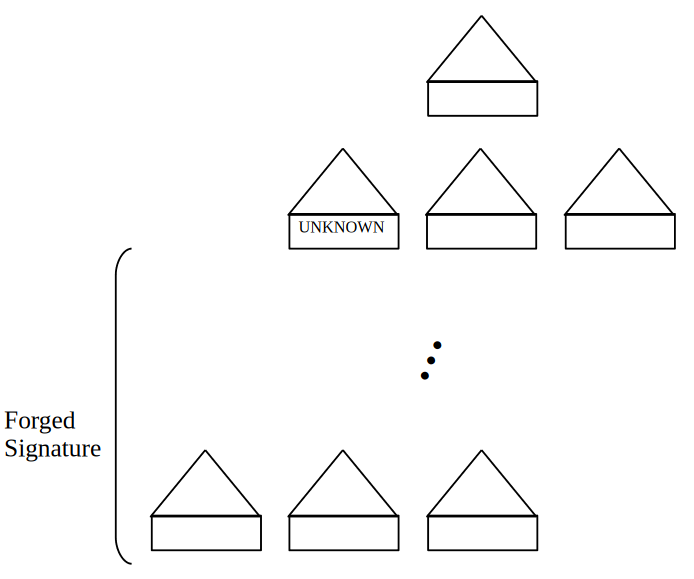
\includegraphics[width=0.5\linewidth]{fig/inter_secr_guess.png}
    \caption{Intermediate Value Guessing}
    \label{fig:intermediateValueGuessing}
\end{figure}

\subsection{Antonov's Attack}

\begin{figure}
    \centering
    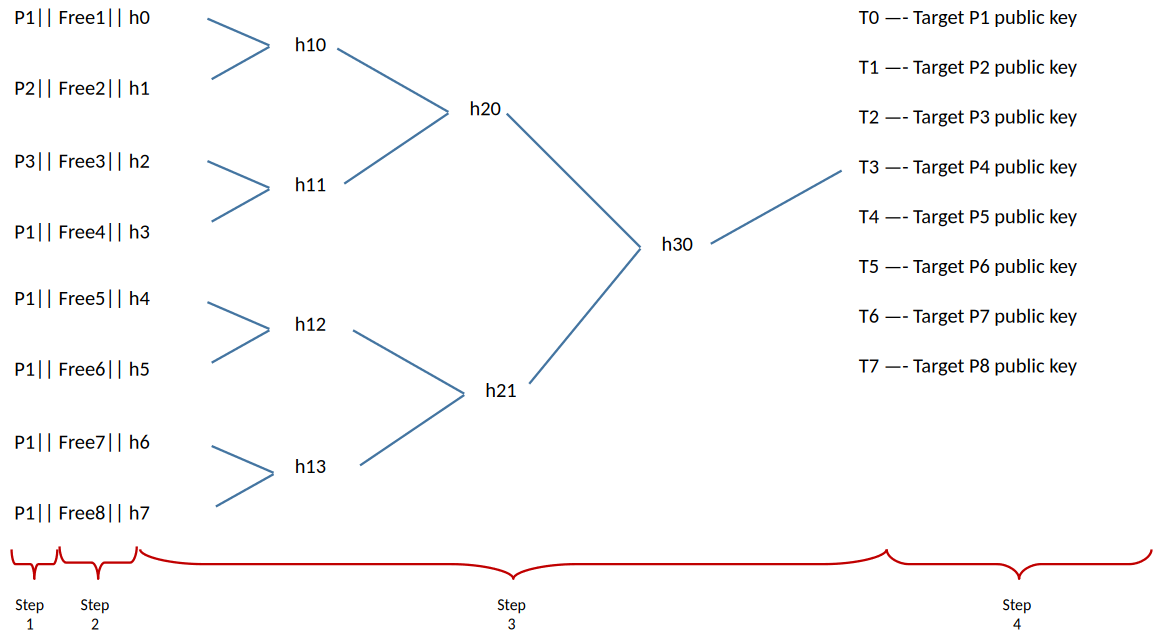
\includegraphics[width=\linewidth]{fig/antonov.png}
    \caption{Antonov's Attack}
    \label{fig:antonov}
\end{figure}

    The attack described in \cite{perlner2022breaking} exploits the Merkle–Damgård construction of the SHA-256 algorithm. Assume there are six target messages \( M_0, \ldots, M_5 \). For each message, different address values \( \text{ADRS}_0, \ldots, \text{ADRS}_5 \) are used within the hash algorithm. At this stage, intermediate values of the compression function \( C \) are obtained for each address.

Then, by applying a collision attack, the adversary finds random values \( x_0, \ldots, x_5 \), and captures pairwise collisions for the next set of intermediate values.

At this point, using the randomly found values \( X_{0,1}, X_{2,3}, X_{4,5} \), a 3-branch collision is constructed.

As the final step, the adversary finds a value \( Z \) such that the following equation holds for some \( i \in \{0,\ldots,5\} \):
\[
\text{SHA-256}(\text{ADRS}_i \,\|\, x_i \,\|\, X_{j,k} \,\|\, Z) = \text{SHA-256}(\text{ADRS}_i \,\|\, M_i)
\]

For example, if the prediction is found for \( M_3 \), then the equation
\[
\text{SHA-256}(\text{ADRS}_3 \,\|\, x_3 \,\|\, X_{2,3} \,\|\, Z) = \text{SHA-256}(\text{ADRS}_3 \,\|\, M_3)
\]
is satisfied, thus completing the multi-target prediction attack.

The complexity of finding a prediction in the final stage for \( t \) target messages is approximately \( 2^{256}/t \) compression function calls. The cost of finding an \( n \)-way collision is also determined by the number of \( C \) function evaluations.

This attack is broken down into four stages, as illustrated in Figure \ref{fig:antonov} 

\paragraph{Step 1:}
In this phase, the adversary collects a number of message-signature pairs signed using the same hash-based signature algorithm. Since the WOTS+ public keys used in the signature can be derived from the signature itself, the adversary also obtains these public keys. The attacker prefers messages with low checksum values at this stage (as lower checksums increase the probability of having \( F \) digits in the base-\( w \) representation). Although all message-signature pairs share the same \( \text{PK.seed} \), each has a distinct ADRS. In Figure~\ref{fig:collision_steps}, \( P_1, \ldots, P_8 \) represent the ADRS and PK.seed values. Finally, the attacker sorts these values.

\paragraph{Step 2:}
Here, the attacker selects random values \( \text{sk}_1, \ldots, \text{sk}_n \) and computes their hashes \( 2w \) times. By concatenating these values, they obtain the aggregated WOTS+ public keys denoted as \( \text{free}_1, \ldots, \text{free}_8 \).

\paragraph{Step 3:}
The attacker appends random values \( h \) to the free values and uses the method explained at the beginning of this section to find an \( n \)-way collision. Unlike Stage 2, the attacker does not know the secret keys corresponding to the WOTS+ public keys in this step.

\paragraph{Step 4:}
In this stage, the attacker compares the found \( n \)-way collision value with the targeted public keys using the value \( h_{30} \). \( T_0, \ldots, T_7 \) represent the target public keys before the checksum is added. If a collision is detected, the attacker has successfully forged a new WOTS+ public key whose hash value matches that of a legitimate public key.

As a result of the above steps, the attacker can generate a forged signature with a fake key. In both SPHINCS+ and XMSS algorithms, public keys generated at each layer during verification are not checked directly—instead, their hash values are computed and passed on to the next layer. Therefore, even if the attacker’s keys differ from the legitimate keys, verification succeeds as long as the hash values match. The main constraint of this attack is that the message to be signed must follow a specific format:

\begin{center}
\texttt{XXXXXXXX XXXXXXXX XXXXXXXF FFFFFFFF FFFFFFFF FFFFFFFF FFFFFFFF FFFFFFFF}
\end{center}

(where \( X \) can be any value). This requirement arises because the attacker knows the secret keys corresponding to the public keys used in Stage 2, but not those in Stage 3. In WOTS+ signatures, the public key is used to sign positions marked with \( F \); therefore, message segments where the secret key is unknown must be fixed to \( F \) to successfully carry out the attack.

\subsection{Fault Injection Attacks}

Fault injection attacks consist of scenarios in which one or more components of the algorithm are assumed to malfunction or operate incompletely due to external interference. For hash-based signature schemes, an example of a fault injection attack is described in the \cite{wagner2023faulting}.

The WOTS+ one-time signature algorithm divides the message to be signed into $w$-bit chunks and generates the signature value by repeatedly applying the hash function to the secret key as many times as the numerical value of each chunk. At this stage, an attacker can compute the hash of the signature value one more time (when the message is not $F$) to create a valid signature. To prevent this, a checksum value is appended to the message before signing. This checksum is calculated as $c = (w - 1 - m)$, where $m$ is the number of $w$-bit message chunks.

With this checksum, if the attacker computes extra hashes from the signature value, the checksum value decreases. Since the hash functions are designed to be resistant to preimage attacks, the attacker cannot compute the new checksum value. The attack described in \cite{wagner2023faulting} is based on the checksum calculation process malfunctioning due to an injected fault. If the checksum calculation does not work correctly, the attacker may generate a valid signature for a message of their choice.

\subsection{Multi-Target Attacks}

Multi-target attacks aim to find preimages when multiple output values of the used hash function are known. For a hash function with an $n$-bit output, the complexity of finding a preimage is $2^n$. In multi-target attacks, if $d$ different hash outputs are known, the complexity of finding a preimage reduces to $2^n / d$.

The XMSS and SPHINCS+ algorithms mitigate this situation by using keyed hash functions. In each usage of the hash function, different key and mask values are used, effectively differentiating the hash function for each operation and ensuring security against multi-target attacks.



\end{section}

\section{Conclusion}

Hash-based signature schemes provide a mature and theoretically sound foundation for post-quantum digital signatures. Their security is grounded in the robustness of cryptographic hash functions, making them well-suited for a future where quantum adversaries may render traditional public-key cryptosystems obsolete. 

In this paper, we presented a comprehensive overview of hash-based signature constructions, starting from early schemes like Lamport and Merkle signatures to standardized schemes such as XMSS and the stateless SPHINCS+. We analyzed their structural differences, key components, and operational procedures, including signature generation, verification, and the role of one-time signatures like WOTS and FORS. We also discussed several cryptanalytic threats specific to HBS schemes, including multi-target attacks, intermediate value recovery, and fault injection attacks, emphasizing the need for implementation-level countermeasures, especially in embedded environments.

As standardization efforts continue and implementation challenges are addressed, hash-based signature schemes are expected to play a central role in securing critical systems, firmware, and communications in the post-quantum era. Future work may focus on improving efficiency, reducing signature sizes, and designing hybrid systems that combine the strengths of HBS with other post-quantum approaches to achieve broader applicability and resilience.


\newpage

\printbibliography

\end{document}